\documentclass[11pt]{article}

\usepackage[a4paper,margin=2.25cm]{geometry}
\usepackage{amsmath,amssymb,amsthm,mathtools}
\usepackage{booktabs}
\usepackage{enumitem}
\usepackage{microtype}
\usepackage{xcolor}
\usepackage{hyperref}
\usepackage{tikz}
\usetikzlibrary{arrows.meta,positioning,fit}

\hypersetup{
  colorlinks=true,
  linkcolor=blue!55!black,
  citecolor=blue!55!black,
  urlcolor=blue!55!black
}

\newtheorem{theorem}{Theorem}[section]
\newtheorem{proposition}[theorem]{Proposition}
\newtheorem{definition}[theorem]{Definition}
\newtheorem{example}[theorem]{Example}
\newtheorem{remark}[theorem]{Remark}
\newtheorem{obligation}[theorem]{Open obligation}

\newcommand{\Rel}{\mathsf{Rel}}
\newcommand{\Comp}{\mathsf{Completion}}
\newcommand{\View}{\mathsf{View}}
\newcommand{\Policy}{\mathsf{Policy}}
\newcommand{\Outcome}{\mathsf{Outcome}}
\newcommand{\Receipt}{\mathsf{Receipt}}
\newcommand{\Source}{\mathsf{Source}}
\newcommand{\Lean}{\textsc{Lean}}

\title{Open-Ended Plural Intelligence:\\
Individuation, Conserved Distinctions, and Relational Coordination}
\author{Oru\v{z}i \and Zarathustra Goertzel}
\date{Working paper, August 2026}

\begin{document}
\maketitle

\begin{abstract}
An open-ended intelligence must act through bounded observations without mistaking
those observations for the world, retain its organization while changing, and
coordinate with agents whose views need not converge.  We present a reusable formal
architecture for these requirements.  Its primitive objects are typed completion
fibres, observer-indexed distinctions, proof-relevant relations between views, and
recoverable evidence.  Cardinal variety, functional translations, compact contexts,
and executable fast paths are derived only when the relevant witnesses exist.

The central no-go result says that a fixed context which remains sufficient for an
accumulated state-separating query schedule must be injective.  Consequently, no
genuinely lossy permanent summary is sufficient for every future policy of an
open-ended agent.  The constructive counterpart is a canonical weakest sufficient
view for every finite active query family, refreshed from recoverable evidence rather
than recursively summarized.  We connect this result to formal accounts of
distinction conservation, relational closure, processual individuation,
variety-under-constraint, metasystem transitions, stigmergy, protected freedom, and
source-scoped adaptive realization.

The development is mechanized in Lean 4.  Positive witnesses and destructive
controls distinguish exact presentations from lossy readouts, relational transport
from earned functionality, individuation from static closure, and semantic admission
from profitability or cache residence.  The resulting theory is general mathematics;
Prime DTT, GSLT-IL, MeTTa spaces, WM-style world models, and self-modifying cognitive
architectures enter as theorem-backed instances rather than defining the theory.
\end{abstract}

\section{The problem: bounded views in an unbounded life}

A cognitive system never carries the whole world in its active context.  It sees a
view, acts, receives new evidence, changes its policies, and often changes the very
language in which it describes the problem.  Three tempting simplifications are
therefore unsafe:

\begin{enumerate}[label=(\arabic*)]
\item treating one compact summary as permanently sufficient;
\item identifying a relation between viewpoints with a function before totality and
      determinism have been established;
\item identifying the persistence of an agent with the persistence of one process,
      prompt, model, or data representation.
\end{enumerate}

The alternative developed here starts from informative objects and derives their
lossy readouts.  The main dependency direction is

\begin{center}
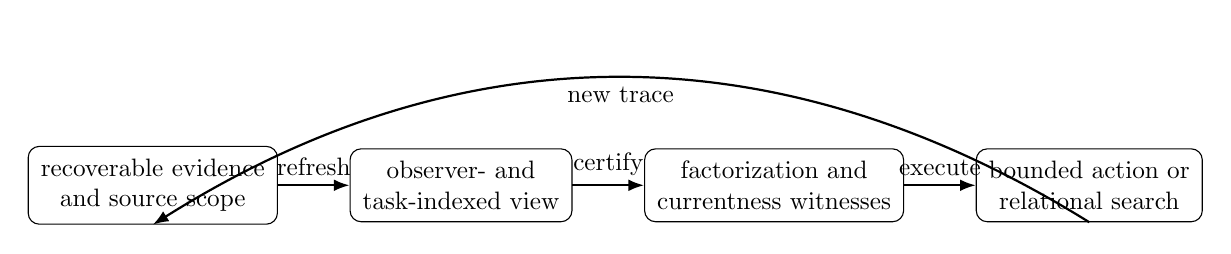
\begin{tikzpicture}[scale=.91,transform shape,
  node distance=7mm and 10mm,
  box/.style={draw,rounded corners,align=center,inner sep=5pt},
  arr/.style={-{Latex[length=2mm]},thick}
]
\node[box] (evidence) {recoverable evidence\\and source scope};
\node[box,right=of evidence] (view) {observer- and\\task-indexed view};
\node[box,right=of view] (cert) {factorization and\\currentness witnesses};
\node[box,right=of cert] (act) {bounded action or\\relational search};
\draw[arr] (evidence) -- node[above]{refresh} (view);
\draw[arr] (view) -- node[above]{certify} (cert);
\draw[arr] (cert) -- node[above]{execute} (act);
\draw[arr,bend right=32] (act.south) to node[below]{new trace} (evidence.south);
\end{tikzpicture}
\end{center}

This is not a proposal to store all history in every hot path.  It separates an
authoritative, persistent source from the small view needed by the present task.
When a policy changes, the system either proves that the policy still factors through
the current view, or refreshes from the source, or uses an exact fallback.

The intellectual sources are complementary.  Heylighen's distinction conservation,
relational closure, constrained variety, metasystem transitions, and stigmergy supply
formal questions about loss, level formation, and mediated coordination
\cite{heylighen1989,heylighen1990,heylighen1995,heylighen2015}.  Weinbaum's account of
becoming and Weinbaum--Veitas's account of open-ended intelligence motivate treating
individuation as a process rather than a static label
\cite{weinbaum2015,weinbaum2018,weinbaumveitas2015}.  Veitas and Weinbaum's ``world of
views'' motivates plural coordination without an assumed global representation
\cite{veitasweinbaum2014,veitasweinbaum2015}.  The definitions and bridge theorems
below are our formal constructions; citations identify the source of the motivating
idea, not a claim that the source already proved the Lean theorem.

\section{Informative objects before numerical readouts}

\subsection{Typed completion fibres}

Let $W$ be a type of worlds and let a statement be a predicate $s : W \to
\mathsf{Prop}$.  Its compatible completions are retained as a type:

\begin{definition}[Completion fibre]
\[
  \Comp(s) \;:=\; \{w : W \mid s(w)\}.
\]
\end{definition}

This type contains the compatible worlds themselves.  A finite cardinality such as
$|\Comp(s)|$ is a derived observation.  If $s_1$ is stronger than $s_2$, every
completion of $s_1$ embeds into the completions of $s_2$.  The Lean development
proves this contravariant embedding before proving its finite cardinal consequence.

The order matters.  Two statements can have equally many completions while admitting
different completions.  A number cannot transport a future witness, explain why an
option is available, or retain provenance.  The fibre can.

\begin{proposition}[Exact presentation]
If two presentations of a completion problem are related by an equivalence that
preserves the underlying membership judgment, then their completion fibres are
equivalent.  When the fibres are finite, their cardinalities are equal.
\end{proposition}

This is the formal basis for comparing presentations without asserting that every
quantity is representation-independent.

\subsection{Observer-indexed variety}

An observer is a function $o : W \to V$.  It distinguishes two worlds when their
observations differ, and its informative variety is the image type
\[
  \mathsf{Variety}(o) := \{v : V \mid \exists w,\; o(w)=v\}.
\]
The fibre above $v$ is $\{w : W \mid o(w)=v\}$.  Thus the theory retains both what the
observer sees and which states the observation identifies.

\begin{theorem}[Observer relativity]
There is no observer-independent finite cardinality of variety in general.  In the
formal control, a micro-observer sees both Boolean coordinates and a macro-observer
forgets the second.  Their observed cardinalities are four and two, respectively.
\end{theorem}

This theorem is intentionally small.  Its role is to prevent a large architectural
error: a later ``variety'' score must name the observer and domain over which it was
measured.

\section{Distinction conservation as a semantic gate}

For source and target distinction relations $D_S$ and $D_T$, a map $f:S\to T$
conserves distinctions when
\[
  D_S(x,y) \Longrightarrow D_T(f(x),f(y)).
\]
When both distinctions are inequality, distinction conservation is exactly
injectivity.  This recovers a precise core of Heylighen's causality-as-distinction-
conservation proposal without identifying every causal question with injectivity
\cite{heylighen1989}.

The useful case is observer-indexed.  A transform may safely erase differences that
a declared observation cannot see, but it may not erase differences on an observable
that a later policy uses.  This makes the gate task-relative without making it
arbitrary.

\subsection{Answer effects}

The GSLT execution layer already distinguishes an answer representation from its
effect on an answer container.  The formalization proves:

\begin{theorem}[Faithfulness criterion]
For an answer effect, conservation of answer distinctions is equivalent to the
existing independently defined faithfulness property.
\end{theorem}

The equivalence prevents a new slogan from becoming a parallel foundation.  It also
classifies two real losses:

\begin{itemize}
\item list-to-bag conversion preserves multiplicity but destroys order;
\item bag-to-support conversion preserves truth support but destroys multiplicity.
\end{itemize}

Concrete collision witnesses prove both failures.  By contrast, decorating every
answer occurrence with a revision identifier conserves the original distinctions.

\begin{remark}[No universal ``dedup is harmless'']
Deduplication may be correct for a support-valued observer and incorrect for a
proof-occurrence-valued observer.  The admissibility theorem must name the observation;
answer-set equality alone is not a universal performance license.
\end{remark}

\section{Closure and individuation}

\subsection{Law-bearing relational closure}

A relational-closure system consists of a network domain, a closure operation, and
proofs of extensivity, monotonicity, and idempotence.  It induces a standard
mathematical closure operator.  The formal object also retains proof-relevant receipts
for connections generated by closure.

This follows the purpose of Heylighen's relational closure: suppress low-level
internal distinctions while making higher-level external distinctions available
\cite{heylighen1990}.  The Lean theory makes the loss explicit.  A seed network and
its closure can be distinct presentations that induce the same closed network.

\begin{example}[Symmetric closure]
Starting from the one-way Boolean edge $\mathsf{false}\to\mathsf{true}$, symmetric
closure adds the reverse edge.  The reverse edge has a generated-connection receipt;
it is absent from the seed.  The seed and the closed presentation nevertheless have
the same closure.
\end{example}

Thus closure is a lawful abstraction, not an identity claim.

\subsection{Individuation is a process}

The general individuation theory separates four objects:

\begin{enumerate}
\item a theory of system states, boundaries, and admissible steps;
\item a static individuated state satisfying closure at a boundary;
\item a proof-relevant process connecting states through steps;
\item persistence, which relates a process to a protected observation.
\end{enumerate}

Processes compose.  ``Becoming individuated'' requires both a process and an
individuated endpoint.  Static closure alone does not manufacture a process.

\begin{theorem}[WM-style instance]
The existing Markov-logic individuation structure, augmented by its explicit
non-emptiness premise, is equivalent to an instance of the general static
individuation theory.  Existing dynamic-individuation paths induce general
individuation processes and persistence results under their stated model assumptions.
\end{theorem}

This recovers rather than replaces the earlier world-model machinery.  It also gives
a precise interpretation of Weinbaum and Veitas's proposal: the identity of an open
agent is carried by an organized transformation process, not by a frozen state
\cite{weinbaumveitas2015,weinbaum2018}.

\subsection{When does a process warrant a new generation?}

An enactive generation is not inferred from closure alone.  It requires a task
interpretation that maps the individuation process to a parent/child policy relation
and proves the relevant completion inclusion.  The development contains both a
positive process-to-generation construction and a negative static shell which is
closed but supplies no generation witness.

This boundary is important: a hierarchy of abstraction levels should be earned by a
semantic transition, not introduced merely because a new type name is convenient.

\section{Constraint, variation, and metasystem transitions}

A constraint on states is a predicate; its fibre is the subtype of states satisfying
it.  Refinement of constraints induces an embedding of fibres.  Separately, a
proof-relevant relation between configurations is classified by totality and endpoint
determinism.  This yields independent axes for:

\begin{center}
constraint present/absent $\times$ static variety/unitarity $\times$
dynamic variation/rigidity.
\end{center}

The eight cases are represented by constructors rather than inferred from prose.
The theory supplies a positive organization with constraint, static variety, and
dynamic variation, and a null organization lacking all three.  This mechanizes the
classification proposed in Heylighen's treatment of systems as constraints on
variety \cite{heylighen1995}.

\begin{definition}[Metasystem transition]
A metasystem packages lower-level systems, admissible variation among them, a
higher-level constraint on that variation, and a task interpretation explaining why
the resulting organization constitutes a new generation.
\end{definition}

The completion fibre of the higher constraint is equivalent to the admissible
higher-level configurations.  A concrete transition is constructed.  A separate
negative theorem shows that mere aggregation plus an external selector is
insufficient: it provides neither internally organized variation nor the task witness
needed for level introduction.

This is a conservative use of the historical idea.  We do not claim that every
evolutionary metasystem transition is captured by the present schema; the schema
isolates a theorem-level condition usable by language and agent architectures.

\section{A world of views: relation first, function earned}

Suppose each viewpoint $i$ has a state type $S_i$.  A coordination route from $i$ to
$j$ is taken primarily to be proof-relevant:
\[
  R_{ij} : S_i \to S_j \to \mathsf{Type}.
\]
It may be partial, branching, or carry multiple witnesses between the same endpoints.
A functional translation $S_i\to S_j$ is derived only when the relation is total and
proof-relevantly endpoint-deterministic.

\begin{theorem}[Representability boundary]
A functional transport exists exactly when every source has a target and all
proof-relevant derivations from a source agree on the target.  The selected function
retains a witness that its graph lies in the original relation.
\end{theorem}

The plural example has one request view and two distinct compatible responses.  It is
open and coordinating, yet admits no functional request-to-response map.  Its reverse
route is functional.  This makes non-convergence a positive architecture rather than
a failed attempt at translation, following the direction proposed by Veitas and
Weinbaum \cite{veitasweinbaum2014,veitasweinbaum2015}.

\subsection{Local coherence need not glue globally}

The cognitive-architecture bridge uses real rational pair charts.  It constructs
pairwise-compatible local marginals which have no global classical joint realization.

\begin{theorem}[No total gluer from local coherence]
There is no function which turns every locally coherent family in the example into a
global realizing chart.
\end{theorem}

This does not license inconsistency by fiat.  It says that the right output of a
failed gluing problem is a contextual family with its local witnesses and obstruction,
not fabricated global consensus.

\section{Stigmergy as trace-mediated coordination}

Following Heylighen, the formal interface names five components: agent, action,
medium, trace, and coordination \cite{heylighen2015}.  A delayed stigmergic episode
requires an earlier action to leave a persistent trace in the medium and a later
action to depend on that trace.

The theory deliberately includes Bateson's natural control: a medium may permit
direct coordination while failing to expose any persisted trace.  Such a medium
cannot construct the stipulated delayed stigmergic episode.  Therefore the definition
does not collapse all coordination into stigmergy.

The MeTTa instance uses an actual proof-relevant space.  Publishing an occurrence
leaves a trace; a later query returns a derivation witnessing that occurrence.  The
space is consequently a coordination medium, not merely a set-valued store.  Order,
multiplicity, and provenance remain observable where the query discipline requests
them.

\section{The open-ended context theorem}

Let $S$ be the recoverable evidence state, $Q$ a type of queries, and $A$ a type of
answers.  A query $q$ denotes $q:S\to A$.  For a finite active set $F\subseteq Q$,
define the canonical active view
\[
  \pi_F(s) := (q(s))_{q\in F} \in \prod_{q\in F} A.
\]

\begin{theorem}[Weakest sufficient finite view]
The active-answer vector $\pi_F$ is sufficient for every query in $F$.  If another
view $v:S\to V$ is sufficient for every query in $F$, then $\pi_F$ factors through
$v$.  Thus $\pi_F$ is the coarsest, or weakest, view sufficient for the declared
query family.
\end{theorem}

When $A$ and $F$ are finite, the representation has the exact ambient bound
\[
  |A|^{|F|}.
\]
This is not a claim that all answer vectors occur; it is the size of the canonical
function space.

Now let $F_0\subseteq F_1\subseteq\cdots$ be an accumulated query schedule.  Say it
separates states when every unequal pair is distinguished at some epoch.

\begin{theorem}[No permanent lossy context]
If a fixed view $v:S\to V$ remains sufficient at every epoch for an accumulated
state-separating query schedule, then $v$ is injective.  Hence no non-injective fixed
context is permanently sufficient for an open-ended separating policy family.
\end{theorem}

The result permits a different decoder at every epoch.  The obstruction is not a
poor decoder; it is permanent information loss.

\begin{example}[Unbounded evidence, two-valued epoch views]
Take $S=\mathbb{N}$ and one Boolean bit-query per epoch.  Every individual epoch view
has exactly two possible answers, while the accumulated schedule separates every
natural number.  A constant permanent context is formally impossible as a sufficient
view, even though each current query is tiny.
\end{example}

The constructive architecture retains $S$ as recoverable evidence and regenerates
$\pi_F$ whenever $F$ changes.  It never recursively summarizes a summary.  This
explains how bounded active context and open-ended intelligence can coexist.

\section{Three freedoms and protected self-transformation}

The formalization keeps three notions apart:

\begin{align*}
\text{semantic freedom} &:= \Comp(p),\\
\text{epistemic latitude} &:= \{s' \mid o(s')=o(s)\},\\
\text{executable freedom} &:= \{c:\Comp(p) \mid c\text{ has a current receipt}\}.
\end{align*}

More compatible refinements can be valuable; more states hidden by an observer can be
mere ignorance; more currently executable actions can be unsafe.  None of the three
numbers subsumes the other two.

A self-modification carries a protected family $P$ of completions.  A valid
transformation supplies a map from every protected pre-modification completion to a
post-modification completion, plus current authority.  Proof-backed weakening yields
such a map constructively.  The Gödel-style architecture bridge proves protected
observation agreement using its existing dynamic-individuation assumptions.

\begin{proposition}[Unconstrained cardinality is unsafe]
Maximizing the number of completions without a protected family can prefer a vacuous
or unsafe weakening.  A concrete finite counterexample has strictly more completions
after weakening while losing a declared protected property.
\end{proposition}

Thus option preservation is relative to a correctness fibre and a protected family,
not a universal instruction to maximize nondeterminism.

\section{Source-scoped adaptive native realization}

Fast execution is licensed by four separate judgments:

\begin{enumerate}
\item \emph{semantic sufficiency}: the requested policy factors through the key;
\item \emph{distinction contract}: the key conserves the distinctions named by the
      requested observation;
\item \emph{currentness}: the source and authority revisions still match;
\item \emph{profitability and retention}: preparation is worth its cost and the plan
      is resident.
\end{enumerate}

Only the first three affect semantic activation.  Profitability may rank or select an
already valid realization; it cannot mint truth.  Cache residence is an operational
fact, not a semantic verdict.

\begin{definition}[Semantic admission]
A prepared realization is semantically admissible when its key supports the policy,
its explicit source/key relation conserves the requested distinctions, its observable
result agrees with the raw result, and an exact raw fallback remains available.
\end{definition}

The Prime/GSLT bridge proves that a current source-scoped receipt induces semantic
admission.  The Cost bridge proves that the identity key on a proof-relevant
elaboration supports every request.  Negative controls show:

\begin{itemize}
\item a constant key can support a constant policy while failing exact distinction
      conservation;
\item support erasure identifies a one-occurrence bag with a two-occurrence bag;
\item a stale revision blocks activation but leaves exact fallback available;
\item overlapping evidence sources do not by themselves establish independence.
\end{itemize}

This yields the implementation shape

\begin{center}
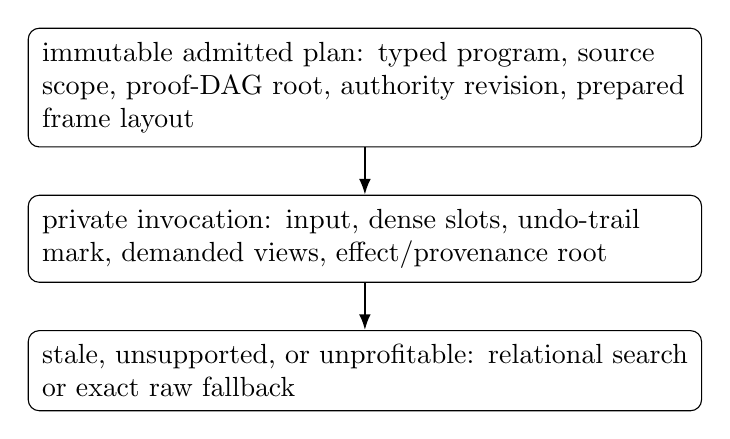
\begin{tikzpicture}[
  node distance=6mm,
  box/.style={draw,rounded corners,align=left,inner sep=5pt,text width=8.2cm},
  arr/.style={-{Latex[length=2mm]},thick}
]
\node[box] (plan) {immutable admitted plan: typed program, source scope,
proof-DAG root, authority revision, prepared frame layout};
\node[box,below=of plan] (inv) {private invocation: input, dense slots, undo-trail
mark, demanded views, effect/provenance root};
\node[box,below=of inv] (fallback) {stale, unsupported, or unprofitable:
relational search or exact raw fallback};
\draw[arr] (plan) -- (inv);
\draw[arr] (inv) -- (fallback);
\end{tikzpicture}
\end{center}

The mathematics does not prescribe a cache policy.  It states what any cache policy
must preserve.

\section{Open-system extension}

An open cognitive language must admit new declarations, rules, views, and execution
realizations without silently changing old meanings.  The GSLT extension boundary
therefore separates authored composition from validated composition.

\begin{theorem}[Current validated growth]
A validated presentation extension with a current dependency receipt transports every
old checked judgment while preserving its protected goal and exact derivation.
\end{theorem}

Two layers may be individually admitted and their authored merge may be syntactically
available while the combined system is invalid.  A validated composite consequently
requires revalidation of the merge.

\begin{theorem}[Boundary crossing requires revalidation]
There exist individually admitted layers whose authored merge is incompatible and
has no validated-composite witness.  Failure to validate the extension does not refute
the source system.
\end{theorem}

This is the conservative-growth rule for Prime/GSLT: old checked meaning is transported
by proof; new joint structure earns admission at the boundary.  The construction has
no finite-vocabulary premise.

\section{Consequences for Prime, GSLT-IL, and cognitive architectures}

The general theory imposes the following dependency order.

\begin{center}
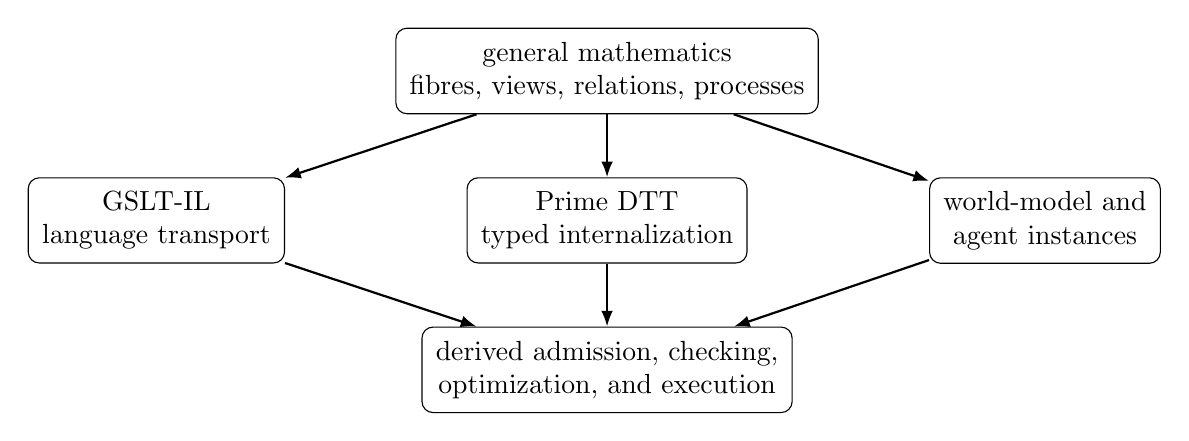
\begin{tikzpicture}[
  node distance=8mm and 14mm,
  box/.style={draw,rounded corners,align=center,inner sep=5pt},
  arr/.style={-{Latex[length=2mm]},thick}
]
\node[box] (math) {general mathematics\\fibres, views, relations, processes};
\node[box,below left=of math] (gslt) {GSLT-IL\\language transport};
\node[box,below=of math] (prime) {Prime DTT\\typed internalization};
\node[box,below right=of math] (wm) {world-model and\\agent instances};
\node[box,below=of prime] (nik) {derived admission, checking,\\optimization, and execution};
\draw[arr] (math) -- (gslt);
\draw[arr] (math) -- (prime);
\draw[arr] (math) -- (wm);
\draw[arr] (gslt) -- (nik);
\draw[arr] (prime) -- (nik);
\draw[arr] (wm) -- (nik);
\end{tikzpicture}
\end{center}

Prime is not defined as an authority checker.  It is a candidate internal language
for the typed completion, relation, evidence, and protected-transformation structures.
GSLT-IL provides proof-relevant language routes, with functions as represented special
cases.  NIK-style authority, compilation, caching, and cost are downstream consumers.
CeTTa or another runtime may implement the settled semantics directly and establish
conformance without becoming the definition of the theory.

For cognitive architectures, identity is the continuing organization of protected
commitments, authoritative memories and receipts, executable capabilities, and the
process that reconstructs task-relative views.  A restart may preserve that
organization; a continuously running process may lose it.  Multi-agent spaces retain
local views and compatibility witnesses, glue only when a certificate exists, and use
persistent traces for delayed coordination.

\section{What has and has not been established}

The mechanized development establishes the theorem families summarized in
Table~\ref{tab:formal-map}.  It does not establish a universal theory of intelligence,
a globally optimal view-selection policy, or a complete operational adequacy theorem
for every runtime.

\begin{table}[ht]
\centering
\small
\begin{tabular}{p{0.23\linewidth}p{0.38\linewidth}p{0.30\linewidth}}
\toprule
Theme & Positive result & Destructive control \\
\midrule
Completion and variety & typed fibres; exact-presentation equivalence & equal counts need not identify options; observer cardinalities differ \\
Distinction conservation & equivalence with answer-effect faithfulness & order and multiplicity erasures collide \\
Closure and individuation & law-bearing closure; composable becoming process & static closure does not create a generation \\
Metasystems & constrained variation plus task interpretation & aggregation and external selection are insufficient \\
World of views & relational coordination; represented functional route & branching route has no function; local coherence need not glue \\
Stigmergy & proof-relevant space publication/query episode & ephemeral direct coordination lacks delayed trace mediation \\
Open-ended context & weakest active view; permanent sufficiency implies injectivity & constant context fails the separating schedule \\
Protected freedom & protected completion maps under valid modification & cardinal freedom alone can discard a protected property \\
Adaptive realization & sufficiency, distinction, currentness, fallback & constant key, stale receipt, support erasure, source overlap \\
Open extension & exact old-judgment transport under validated growth & individually valid layers can have an invalid merge \\
\bottomrule
\end{tabular}
\caption{Theorem-backed positive and negative boundaries.}
\label{tab:formal-map}
\end{table}

\begin{obligation}[Operational adequacy]
Relate the abstract source-scoped realization receipts to complete runtime receipts,
including work, span, allocation, invalidation, and proof-DAG sharing, without erasing
answer occurrences.
\end{obligation}

\begin{obligation}[Contextual invention]
Extend weakest-sufficient views to open terms and policies under binders.  This needs
contextual codes and substitution coherence; the closed finite-query theorem does not
by itself solve typed predicate invention.
\end{obligation}

\begin{obligation}[Certified parallel composition]
Prove when completion fibres of parallel agents compose as products.  Disjoint source
scope alone is insufficient; resource and communication independence must also be
certified.  Interacting systems generally require a pullback or proof-relevant
relational convolution.
\end{obligation}

\begin{obligation}[Selection under distribution shift]
Compare weakness, description length, and probabilistic selectors while retaining
candidate occurrences, distinct support, runtime cost, and future-task success as
separate measurements.
\end{obligation}

\section{Conclusion}

Open-endedness does not require an infinitely large active context or a single global
world model.  It requires that bounded views remain honest about what they forget,
that richer evidence can be revisited, that translations remain relational until
functionality is earned, and that self-transformation preserves explicitly protected
futures.

The core lesson is simple.  Keep the informative object first: the completion fibre,
the proof-relevant route, the process, the trace, the receipt.  Derive the number,
Boolean, function, cache key, or compact view only with a theorem describing the loss.
That discipline supports plural open systems while still permitting efficient native
execution.

\appendix
\section{Lean theorem map}

The implementation is organized by semantic subject rather than by application.
The principal modules are:

\begingroup
\small\raggedright
\Urlmuskip=0mu plus 1mu\relax
\begin{itemize}
\item \path{Mettapedia/Enactive/CompletionFibre.lean},
      \path{Mettapedia/Cybernetics/ObservedVariety.lean};
\item \path{Mettapedia/Cybernetics/DistinctionConservation.lean},
      \path{Mettapedia/GSLT/Dynamics/AnswerDistinctionConservation.lean};
\item \path{Mettapedia/Cybernetics/RelationalClosure.lean},
      \path{Mettapedia/Cybernetics/Individuation.lean},
      \path{Mettapedia/Logic/MarkovLogicIndividuationBridge.lean},
      \path{Mettapedia/Enactive/IndividuationGeneration.lean};
\item \path{Mettapedia/Cybernetics/ConstrainedVariety.lean},
      \path{Mettapedia/Enactive/MetasystemTransition.lean};
\item \path{Mettapedia/GSLT/Dynamics/WorldOfViews.lean},
      \path{Mettapedia/CognitiveArchitecture/Agent/WorldOfViewsBridge.lean};
\item \path{Mettapedia/Cybernetics/Stigmergy.lean},
      \path{Mettapedia/Languages/MeTTa/StigmergicSpace.lean};
\item \path{Mettapedia/CognitiveArchitecture/Agent/OpenEndedContext.lean};
\item \path{Mettapedia/Enactive/ProtectedFreedom.lean},
      \path{Mettapedia/CognitiveArchitecture/GodelClaw/Ethics/ProtectedFreedomBridge.lean};
\item \path{Mettapedia/Languages/MeTTa/Prime/SourceScopedAdaptiveRealization.lean};
\item \path{Mettapedia/GSLT/LanguageDef/OpenSystemExtensionBoundary.lean}.
\end{itemize}
\endgroup

The historical claims in the paper are not inserted as axioms.  They motivate
definitions; all named project results are checked Lean declarations with explicit
premises.

\begin{thebibliography}{99}

\bibitem{heylighen1989}
Francis Heylighen.
\newblock Causality as distinction conservation: A theory of predictability,
reversibility and time order.
\newblock \emph{Cybernetics and Systems}, 20:361--384, 1989.

\bibitem{heylighen1990}
Francis Heylighen.
\newblock Relational closure: A mathematical concept for distinction-making and
complexity analysis.
\newblock In R. Trappl, editor, \emph{Cybernetics and Systems '90}, pages
335--342. World Scientific, 1990.

\bibitem{heylighen1995}
Francis Heylighen.
\newblock (Meta)systems as constraints on variation: A classification and natural
history of metasystem transitions.
\newblock \emph{World Futures: The Journal of General Evolution}, 45:59--85,
1995.

\bibitem{heylighen2015}
Francis Heylighen.
\newblock Stigmergy as a universal coordination mechanism: Components, varieties
and applications.
\newblock In T. Lewis and L. Marsh, editors, \emph{Human Stigmergy: Theoretical
Developments and New Applications}. Springer, 2015.

\bibitem{weinbaum2015}
David R. Weinbaum.
\newblock Complexity and the philosophy of becoming.
\newblock \emph{Foundations of Science}, 20:283--322, 2015.
\newblock \url{https://doi.org/10.1007/s10699-014-9370-2}.

\bibitem{weinbaum2018}
David R. Weinbaum (Weaver).
\newblock \emph{Open-Ended Intelligence}.
\newblock PhD thesis, Vrije Universiteit Brussel, 2018.

\bibitem{weinbaumveitas2015}
David Weinbaum (Weaver) and Viktoras Veitas.
\newblock Open ended intelligence: The individuation of intelligent agents.
\newblock arXiv:1505.06366, 2015.

\bibitem{veitasweinbaum2014}
Viktoras Veitas and David Weinbaum (Weaver).
\newblock A world of views: A world of interacting post-human intelligences.
\newblock arXiv:1410.6915, 2014.

\bibitem{veitasweinbaum2015}
Viktoras Veitas and David Weinbaum (Weaver).
\newblock Living cognitive society: A digital world of views.
\newblock arXiv:1602.08388, 2016.

\end{thebibliography}

\end{document}
